\paragraph{Finding a preconditioning sequence}
To facilitate emotional conditioning I selected a specialized sequence containing images with a corresponding emotional charge.
Each sequence contains 21 to 39 \todo{more precise} images with each displayed for about 5 seconds.

Each subject is assigned one of four preconditioning sequences. Each sequence is aimed to condition the subject into one of the 4 quadrants, described though a valence-arousal emotional model. To simplify we will label (\ref{fig:valence_arousal_model}) them as:
\begin{enumerate}
	\item Angry (Quadrant 1)
	\item Happy (Quadrant 2)
	\item Sad (Quadrant 3)
	\item Relaxed (Quadrant 4)
\end{enumerate}


\begin{figure}
\begin{center}
	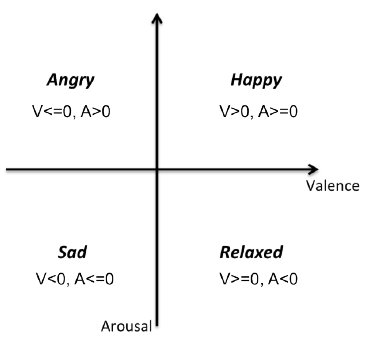
\includegraphics[width=150px]{graphics/Valence-Arousal-model-showing-the-quadrants-of-the-four-emotion-tags-used-in-this_W640.jpg}
	\caption{Valence Arousal Model \cite{Song2013} \label{fig:valence_arousal_model}}
	
\end{center}
\end{figure}

There are several emotional image data-sets available for academic purposes such as GAPED \cite{Dan-Glauser2011}, OASIS \cite{Kurdi2017}, IAPS \cite{Lang1997} and NAPS \cite{Marchewka2014}. While NAPS is offering the highest realism and quality of images, the range images seems to cover "sad" and "happy" to a less pronounced degree. In general, strong negative valence values are accompanied with high arousal values across all analyzed data-sets. Causing sadness is a challenging task. In current preconditioning sequences I am using the \textbf{OASIS} database. It has relatively wide spread of emotions compared to other sets.

Keeping in mind the need for a clear separation between groups in terms of their emotional state into account, I limited emotional images to moderately strong stimuli values, thus avoiding extreme reactions and unrealistic emotional states. It can be assumed that in most cases, people who attend e-learning lessons will have moderate levels of emotional charge. It is important to note that quadrant 1 - angry and quadrant 2 - happy has a more pronounced representation in emotional databases due to an easier and more prevalent stimuli availability. As such quadrant 1 and quadrant 2 have stronger stimuli compared to quadrant 3 and 4. It is expected that there will be a significant difference between emotion ratings of participants across these groups.

It is understood that the e-learning interface under real conditions will only cause mild-to-moderate changes to a mood.


\begin{figure}
	\centering
	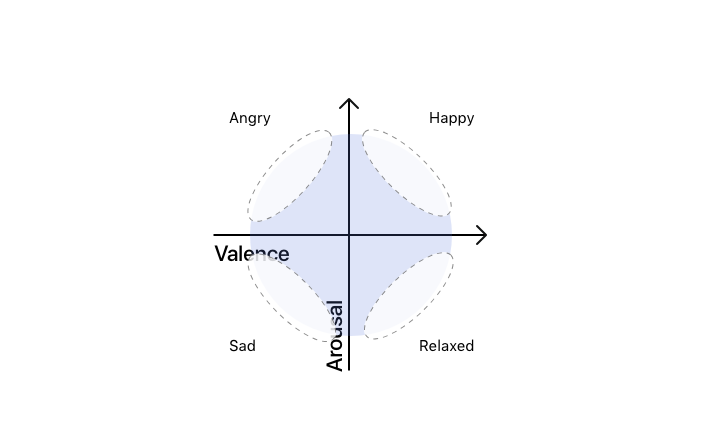
\includegraphics[width=0.7\linewidth]{graphics/Valence-Arousal-Model-1.png}
	\caption{Focus levels of emotional states on valence arousal model}
	\label{fig:valence-arousal-model-2}
\end{figure}

Illustration \ref{fig:valence-arousal-model-2} highlights with dashed outline areas the target arousal and valence values
